
\documentclass[11pt]{article}

\usepackage{fullpage,epsfig,latexsym,picinpar,amsbsy,amsmath,tikz}

\newcommand{\depth}{{\mbox{\it depth}}}
\newcommand{\level}{{\mbox{\it level}}}

\newcommand{\boo}{{\sf boo}}
\newcommand{\foo}{{\sf foo}}
\newcommand{\goo}{{\sf goo}}

\newcommand{\delete}{{\mbox{\tt delete}}}
\newcommand{\decreasekey}{{\mbox{\tt decreasekey}}}
\newcommand{\extractmin}{{\mbox{\tt extractmin}}}


\setlength{\evensidemargin}{0.1in}
\setlength{\oddsidemargin}{0.1in}
\setlength{\textwidth}{6.6in}
\setlength{\topmargin}{0.0in}
\setlength{\textheight}{8.7in}
\setlength{\headheight}{0in}
\setlength{\headsep}{0in}
\setlength{\topsep}{0in}
\setlength{\itemsep}{0in}
\renewcommand{\baselinestretch}{1.1}
\parskip=0.080in
                                                                                                                         
\newcommand{\parend}[1]{{\left( #1  \right) }}
\newcommand{\spparend}[1]{{\left(\, #1  \,\right) }}
\newcommand{\angled}[1]{{\left\langle #1  \right\rangle }}
\newcommand{\brackd}[1]{{\left[ #1  \right] }}
\newcommand{\spbrackd}[1]{{\left[\, #1  \,\right] }}
\newcommand{\braced}[1]{{\left\{ #1  \right\} }}
\newcommand{\leftbraced}[1]{{\left\{ #1  \right. }}
\newcommand{\floor}[1]{{\left\lfloor #1\right\rfloor}}
\newcommand{\ceiling}[1]{{\left\lceil #1\right\rceil}}
\newcommand{\barred}[1]{{\left|#1\right|}}
\newcommand{\doublebarred}[1]{{\left|\left|#1\right|\right|}}
\newcommand{\spaced}[1]{{\, #1\, }}
\newcommand{\suchthat}{{\spaced{|}}}
\newcommand{\numof}{{\sharp}}
\newcommand{\assign}{{\,\leftarrow\,}}
                                                                                                                         
\newcommand{\veps}{{\varepsilon}}
\newcommand{\Sigmastar}{{\Sigma^\ast}}
\newcommand{\barx}{{ \bar x}}

\newcommand{\half}{{\mbox{$\frac{1}{2}$}}}
\newcommand{\threehalfs}{{\mbox{$\frac{3}{2}$}}}





\newcommand{\Union}{\mbox{\sf union}}
\newcommand{\Find}{\mbox{\sf find}}

\pagestyle{empty}
\begin{document}

\centerline{\large \bf CS218 ASSIGNMENT 3}
\centerline{due Thursday, February 21, at 5PM}

\vskip 0.3in
\noindent
\bf{Individual assignment: Problems 1,2}

\noindent
\bf{Group assignment: Problems 1,2,3}

\vskip 0.2in

%%%%%%%%%%%%%%%%%%%%%%%%%%%%

\tikzset {treenode/.style={align=center,inner sep=0pt}}
\tikzset {node_black/.style={treenode,circle,white,font=\bfseries,draw=black,fill=black,text width=0.6cm}}
\tikzset {node/.style={treenode,,circle,draw=black,text width=0.6cm}}
\tikzset {triangle/.style = {regular polygon, regular polygon sides=3 }}
\tikzset {edge from parent/.style={draw,latex-}}


\begin{problem}
Suppose that we are using disjoin-set forests with union by rank and path compression. We start with the forest containing singleton sets $\braced{i}$, for $i = 1,\dots,20$. We execute the following sequence of operations:
%
\noindent
{\small
\begin{eqnarray*}
\begin{array}{lllllll}
\Union(1,2)\quad & \Union(3,4)\quad &\Union(5,6) \quad
    &\Union(7,8)\quad & \Union(9,10) \quad & \Union(11,12)\quad &\Union(13,14) \\
%
\Union(15,16) & \Union(17,18) &\Union(19,20) & \Union(2,4) & \Union(6,8) 
 	& \Union(10,11) & \Union(13,16) \\
%
 \Union(17,20) 	&  \Find(1) & \Union(8,12)  & \Union(14, 20)
	 & \Union(2,17) & \Find(9) &  \Union(13,5)
\end{array}
\end{eqnarray*}
}
%
Draw the forest (a) after $\Union(17,20)$, (b) after $\Union(14,20)$, (c) after $\Union(13,5)$. Assume that whenever we execute $\Union(x,y)$, then we first do $\Find(x)$, $\Find(y)$, and then the union for the roots. (This slightly differs from the lecture.)
\end{problem}

\paragraph{Answer}
(a). After $\Union(17,20)$, union by rank has a same graph as path compression:

\begin{tikzpicture}
    \node[node] at (0,0) {4}
        child{ node [node] {2} 
            child{ node [node] {1} }
        }
        child{ node[node] {3}};
    \node[node] at (3,0) {8}
        child{ node[node] {6}
            child{ node[node] {5}}
        }
        child{ node[node] {7}};
    \node[node] at (6,0) {12}
        child{ node[node] {10}
            child{ node[node] {9}}
        }
        child{ node[node] {11}};
    \node[node] at (9,0) {16}
        child{ node[node] {14}
            child{ node[node] {13}}
        }
        child{ node[node] {15}};
    \node[node] at (12,0) {20}
        child{ node[node] {18}
            child{ node[node] {17}}
        }
        child{ node[node] {19}};
\end{tikzpicture}

(b). After $\Union(14,20)$, union by rank:

\begin{tikzpicture}
    \node[node] at (0,0) {4}
        child{ node [node] {2} 
            child{ node [node] {1} }
        }
    child{ node[node] {3}};
    \node[node] at (6,0) {12}
        child{ node[node] {8}
            child{ node[node] {6}
                child{ node[node] {5}}
            }
            child{ node[node] {7}}
        }
        child{ node[node] {10}
            child{ node[node] {9}}
        }
        child{ node[node] {11}};
    \node[node] at (12,0) {20}
        child{ node[node] {16}
            child{ node[node] {14}
                child{ node[node] {13}}
            }
        }
        child{ node[node] {18}
            child{ node[node] {17}}
        }
        child{ node[node] {19}};
\end{tikzpicture}

Path compression:

\begin{tikzpicture}
    \node[node] at (0,0) {4}
        child{ node [node] {2} 
            child{ node [node] {1} }
        }
    child{ node[node] {3}};
    \node[node] at (6,0) {12}
        child{ node[node] {8}
            child{ node[node] {6}
                child{ node[node] {5}}
            }
            child{ node[node] {7}}
        }
        child{ node[node] {10}
            child{ node[node] {9}}
        }
        child{ node[node] {11}};
    \node[node] at (12,0) {20}
        child{ node[node] {16}
            child{ node[node] {15}}
        }
        child{ node[node] {14}
            child{ node[node] {13}}
        }
        child{ node[node] {18}
            child{ node[node] {17}}
        }
        child{ node[node] {19}};
\end{tikzpicture}

(c). After $\Union(13,5)$, union by rank:

Path compression:

\begin{tikzpicture}
    \node[node] at (6,0) {12}
        child{ node[node] {5}}
        child{ node[node] {11}}
        child{ node[node] {13}}
        child{ node[node] {8}
            child{ node[node] {6}}
            child{ node[node] {7}}
        }
        child{ node[node] {10}
            child{ node[node] {9}}
        }
        child{ node[node] at (4,0) {20}
            child{ node[node] {14}}    
            child{ node[node] {17}}
            child{ node[node] {18}}
            child{ node[node] {19}}
            child{ node[node] {2}
                child{ node[node] {1}}
            }
            child{ node[node] {4}
                child{ node[node] {3}}
            }
            child{ node[node] {16}
                child{ node[node] {15}}
            }
        };
        
\end{tikzpicture}



\begin{problem} \text{(10 points)}
Let {\sf NetFlow} stand for the network flow problem, as covered in class. Consider a generalized network flow problem {\sf NetFlowVC}, in which capacities are defined both for edges and vertices. In this version, the total flow into a vertex cannot exceed the given capacity. Show that {\sf NetFlowVC} can be reduced to {\sf NetFlow}, and that its time complexity is the same.
\end{problem}

%%%%%%%%%%%%%%%%%%%%%%%%%%%%


\begin{problem} \text{(10 points)}
Consider the network below. Use Dinic's algorithm to find the maximum flow in this network. For each phase of the algorithm, except first, you need to show (a) the residual graph before the augmentation, and (b) the layered graph and the flow resulting from the augmentation. At the end, show the final flow and prove that it is indeed maximum.

\noindent
\begin{center}
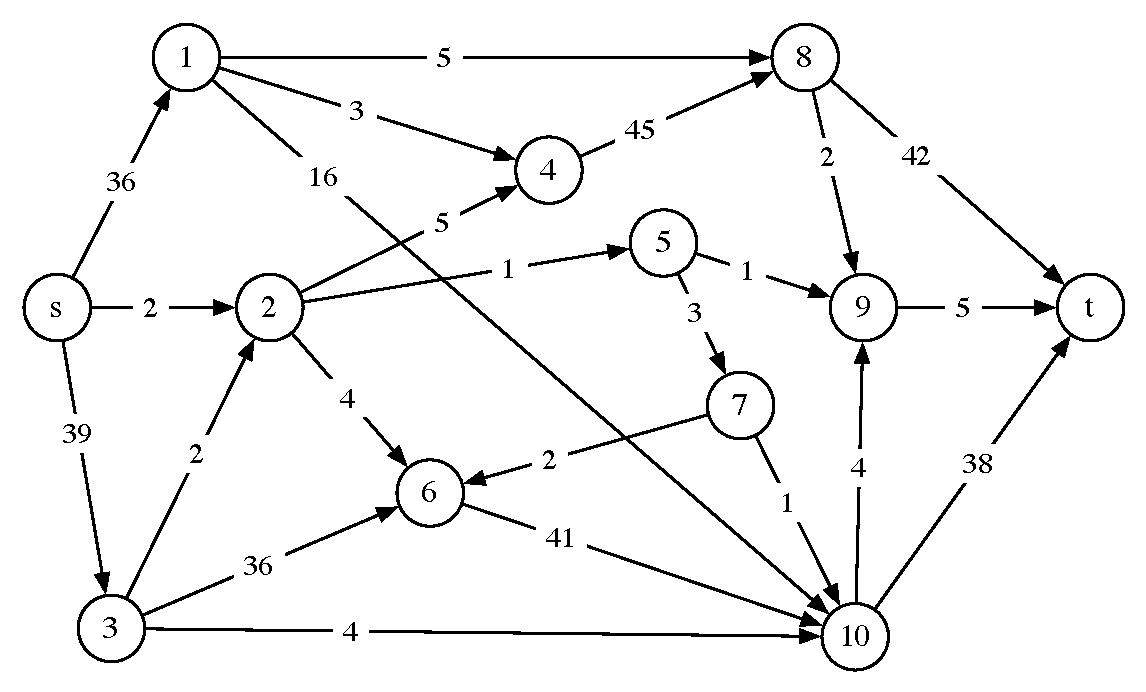
\includegraphics[width=4in]{hw3_dinic.pdf} %
\end{center}
\end{problem}

%%%%%%%%%%%%%%%%%%%%%%%%%%%%

\vskip 0.2in
\section{\text{Submission.}}
\text{Submit the pdf file via gradescope by 5PM on Thursday, February 21. For pair assignments, submit one pdf only with two names on it.}


\end{document}

